\section{Ranking Model}
\label{sec-model}

In this section, we first present Time-Weighted PageRank for evaluating  the importance of entities, defined as a combination of the prestige and popularity, and then introduce our ranking model \ensemblerank that assembles the importance of articles, venues and authors involved in scholarly articles.
%
%\markedb{Before going into details, it is worthy pointing out that although this work focuses on query independent ranking, it can also be used for query dependent ranking. Our ranking can serve as an indicator of the importance of items, and, given a specific query, it can either be directly used to rank a subset of relevant items or combine with any relevance scores.}

%It further assembles the importance of heterogeneous entities involved to rank scholarly articles.
%The model is based on PageRank~\cite{Brin98:PageRank}, which was initially designed for web pages and widely applied to many other tasks, including article ranking~\cite{Li08TSRanking,Richardson06:BPR,sayyadi09,Zhou07-CoRank}.


\subsection{Time-Weighted PageRank}
\label{subsec-twpr}

We first present Time-Weighted PageRank (TWPageRank) based on citation statistics, as the direct use of PageRank for ranking scholarly articles is problematic as discussed below.




%PageRank~\cite{Brin98:PageRank} has been extensively applied to the ranking of scholarly articles~\cite{Waltman2014,sayyadi09,Zhou07-CoRank,ChenXMR07}, as hyperlinks among Web pages can be easily replaced with citation relationships among articles, and citation analysis plays a key role to evaluate the importance of scholarly articles. However,



\noindent(1) Different articles typically have different impacts in practice, and there is a need to differentiate, while PageRank essentially assumes equal impacts.

%, such that each article can distribute more of its authority to those that are more influential to it.

\noindent(2) The semantics of citation relationships are time-dependent, which means that citations at different periods of time may reveal different information. Note that this has already been exploited for scholarly article ranking~\cite{Li08TSRanking,Wang13AAAI,WalkerXKM07}, while PageRank does not consider this temporal factor at all.
% and each individual article reaches their periods in different time

\stitle{Time-Weighted PageRank (TWPageRank)}. Most previous work simply exploits temporal information in the form of exponential decay~\cite{Li08TSRanking,Wang13AAAI,sayyadi09,WalkerXKM07}. We rethink the usage of time information in terms of the impacts of scholarly articles.
Recall that articles are categorized  into six citation patterns featured by the time when the articles reach their citation peaks~\cite{Chakraborty15}: (a) {\em PeakInit} with a single citation-count peak in the first five years (but not the first year) after publication, (b) {\em PeakMul} with distinct multiple peaks, (c) {\em PeakLate} with a single peak in at least five years   (but not the last year) after publication, (d) {\em MonDec} with monotonically decreasing citations, (e) {\em MonIncr} with monotonically increasing citations, and, (f) {\em Other} for articles whose average numbers of citations per year are less than 1. Though the number of citations is an indicator of the impact of an article~\cite{WangSB13,Garfield471}, its impact is time-dependent but not simply in the form of exponential decay that only considers  the case of {\em MonDec}.
%
To unify these distinct citation patterns and to make our ranking model succinct, we adopt that {\em the impact of an article tends to decay with time after the peak time}, as pointed out by the aging function in~\cite{WangSB13}. That is, the impacts of articles directly decay with time only for those in {\em MonDec}, and decay with time after the (highest) peak time for those in {\em PeakInit}, {\em PeakLate} and {\em PeakMul}, and do not decay for ones in {\em MonIncr} (which is rare).
%Otherwise, its impact is fixed as a constant number. %, since we argue that the increment of its citations during this period is mainly due to the increase of its popularity.
Also observe that {\em each individual article has its own peak time} as articles may reach their citation peaks in different patterns and time.
%using the peak year in Fig.~\ref{fig-citation} is not appropriate for all articles. On the contrary, we compute a peak year for each article.


\eat{
 the proportion of total citations \wrt the number of years after publication.
%Here we use the number of citations to evaluate the impacts of articles.
\marked{As we can see, the number of citations reaches a peak in the first 1 or 2 years, and gradually decreases after that, which also conforms to our perception of the impacts of articles~\cite{WangSB13}. Note that the peak time differs from one dataset to another.}


According to Fig.~\ref{fig-citation}, the impact of an article does depend on time, but not simply in the form of exponential decay. Specifically, if an article is cited after the citation peak, its impact should decay with time. Otherwise, its impact is fixed as a constant number. %, since we argue that the increment of its citations during this period is mainly due to the increase of its popularity.
Moreover, considering that articles might reach their citation peaks in different time, we compute {\em the peak time for each individual article}, rather than using the same citation peak for all articles.
%using the peak year in Fig.~\ref{fig-citation} is not appropriate for all articles. On the contrary, we compute a peak year for each article.
}

\begin{figure}
\centering
\hspace{-4ex}
\subfigure{\label{fig-paper}
\includegraphics[scale=0.414]{fig/yearly-papers.eps}}
\hspace{-4ex}
\subfigure{\label{fig-citation}
\includegraphics[scale=0.414]{fig/yearly-references.eps}}
\caption{\small Statistics of scholarly articles: (1) the (logscale) percentage of papers in each year \wrt\ all papers (left) and (2) the (logscale) percentage of citations in each year \wrt\ all citations (right) on datasets \aan, \aminer and \magdata, respectively.}
\label{fig-data-analysis}
\vspace{-3ex}
\end{figure}
%[{\scriptsize a}] [{\scriptsize b}]

Based on the above discussion, we propose TWPageRank that evaluates the prestige of nodes (\eg scholarly articles) in a directed graph, such that each node is attached with time information. It differs from PageRank by weighing the influence propagation using the {\em impact weights on edges}, which represent the relative amounts of time-dependent prestige that should be propagated from the edge sources to targets.
%
Formally, the impact weight on a directed edge $(u,v)$, \ie an edge from $u$ to $v$, is defined as:

\vspace{-1ex}
\begin{small}
\begin{equation} \label{eq-infl-weights}
w(u,v)  =  \begin{cases}  \hspace{7ex} 1 & T_u <  Peak_v \\
  e^{\sigma(T_u-Peak_v)} & T_u \geq Peak_v,
\end{cases}
\end{equation}
\end{small}
%
\noindent where $T_u$ is the time of node $u$, $Peak_v$ is the peak time of node $v$ after which the impact weights of edges to $v$ decay with time, and $\sigma$ is a negative number controlling the decaying speed of the impacts.
By default, Eq.~(\ref{eq-infl-weights}) uses years as its time granularity. Note that the time decaying factor $\sigma$ is introduced to provide flexibility for TWPageRank in various applications, and its value is typically within a small interval, \eg $[-2,0]$, such that $w(u,v)$ does not decay when $\sigma=0$ and already decays more than a half per year when $\sigma=-1$.
%For the sake of completeness, we further set $w(u,v)$ to $0$ if there does not exist an edge from $u$ to $v$ in the graph.


For scholarly article ranking, $T_u$ is the publication time of article $u$ and $Peak_v$ should be ideally set to the time when article $v$ has the highest impact. Basically, it could simply be the year when article $v$ obtains the largest number of citations. However, recent work reveals that the volume of scientific publications and the number of citations grow exponentially with time~\cite{Dong2017KDD,BornmannM15}. We also collect and report the volume and citation statistics on three scholarly datasets in Fig.~\ref{fig-data-analysis}, which verifies the exponential distribution. Hence, we adopt the {\em scaled} number of citations $\Psi_v^{(t)}=\Phi_v^{(t)} / \log Z^{(t)}$ such that $\Phi_v^{(t)}$ and $Z^{(t)}$ are the number of citations of article $v$ at year $t$ and the total number of citations at year $t$, respectively. The peak time $Peak_v$ is the time that maximizes $\Psi_v^{(t)}$.
%(\aan, \aminer and \magdata)
% since scholarly data is dynamic and continuously growing
%, and the increased number of references of each article over time
%Recent work observes that the volume of scientific publications doubled every 12 years between 1900 and 2015~\cite{Dong2017KDD}. It is not surprising that the number of references also grows exponentially~\cite{BornmannM15}.



The update rule of TWPageRank is:

\vspace{-1ex}
\begin{small}
\begin{equation}\label{eq-twpr}
PR(v)=d\sum_{(u,v)\in E} \frac{w(u,v)PR(u)}{W(u)}+\frac{1-d}{n},
\end{equation}
\end{small}
where $PR(u)$ and $PR(v)$ are the TWPageRank scores of $u$ and $v$, respectively, $E$ is the set of edges, $W(u)=\Sigma_{v} w(u,v)$ is the sum of the impact weights on all edges from $u$, $n$ is the number of nodes and $d$ is a damping parameter in $(0, 1)$. By Eq.~(\ref{eq-twpr}), we can see that prestige is updated based on the impact weights, not equally distributed.

% in Eq.~(\ref{eq-twpr}) into
Correspondingly, the matrix form of the update rule is:

\vspace{-1ex}
\begin{small}
\begin{equation}
\label{eq-twpr-update}
PR^{(t)}=d M^T  PR^{(t-1)} + (1-d) e/n.
\end{equation}
\end{small}
%
\noindent
Here $PR^{(k)}$ is the TWPageRank vector after $k$ iterations,  $M$ is the transition matrix such that $M_{u,v}=w(u,v)/W(u)$ and  $e$ is an $n$-dimensional all-one vector $[1]_{n\times1}$.

%We next present the convergence  of TWPageRank as follows.
The linear system in Eq.~(\ref{eq-twpr-update}) is equivalent to {\em irreducible} and {\em aperiodic} Markov chains~\cite{CorsoGR05}, which guarantees the following.


\begin{prop}
\label{prop-converg}
TWPageRank converges to a unique  vector on any graph, regardless of the initial vector.
\end{prop}


\eat{%%%%%%%
\begin{proof}
It is known that a sequence of vectors $x^{(k)}$ such that $x^{(k+1)}=A\cdot x^{(k)}+b$ (where $k=0,1,\dots$) converges to a unique vector $x^*$,  regardless of the initial vector $x^0$, if and only if $\rho(A)<1$~\cite{kelley1999iterative}, where $\rho(A)$ is the spectral radius of matrix $A$. Hence, it suffices to show $\rho(d\cdot M^T) < 1$ by Eq.~(\ref{eq-twpr-update}).

As the column sums of $d\cdot M^T$ are all less than or equal to $d$, $||d\cdot M^T||_1 \le d$ where $||d\cdot M^T||_1$ is the 1-norm of matrix $d\cdot M^T$ and is defined as the maximum absolute column sum of $d\cdot M^T$.
We then have $\rho(d\cdot M^T) \le ||d\cdot M^T||_1 \le d < 1$, as the spectral radius of a matrix is always no more than its consistent matrix norms~\cite{spe-radius}, \eg $||\cdot||_1$, which gives the conclusion.
\end{proof}
}

%\stitle{Remarks}. Note that Eq.~(\ref{eq-twpr}) is indeed a general update rule of Weighted PageRank~\cite{Xing04:WPR,Ding11}, and the name of Time-Weighted PageRank comes from the use of time information of citations in the initial impact weight  $w(u,v)$ of Eq.~(\ref{eq-infl-weights}).

%\vspace{-1ex}
%\stitle{Remarks}.
%\markedb{
%The goal of our TWPageRank is to change node values, \ie importance. One may wonder why not directly change node values. However, it is difficult to handle as importance does not have a clear and closed-form definition and it may also cause problems for convergence.
%To our knowledge, there is no related work on changing node weights and it is yet unclear how to handle it. Finally, we use impact weights to achieve the goal since %importance is essentially propagable through edges and it is also fair for all nodes.
%}

\vspace{-1ex}
\subsection{Ranking with Importance Assembling}
\label{subsec-ensemble}


%In our model, the importance of scholarly articles is defined as a combination of the prestige and popularity of its associated articles, venues and authors. Intuitively, prestige favors those with many citations soon after the publication of articles for citation component or associated articles for venue and author components, and popularity favors those with recent citations. Both prestige and popularity capture the temporal nature of entities in scholarly data.
In our model, the importance is defined as a combination of the prestige and popularity. Intuitively, prestige favors those with many citations soon after the publication of articles or associated articles of venues and authors, and popularity favors those with recent citations. Both prestige and popularity capture the temporal nature of entities. %in scholarly data.

Our ranking model \ensemblerank,  illustrated in Fig.~\ref{fig-rankmodel}, assembles the importance of article, venue and author entities for scholarly article ranking, which is computed by the citation, venue and author components, respectively.
%
We next introduce the details of the three components.


\stitle{Citation component}.
The first component computes the importance of articles using the citation information.

A {\em citation graph} $G^c(V^c, E^c)$ is firstly constructed using the citation information such that (a) a node in $V^c$ denotes an article, (b) a directed edge $(u,v)$ in $E^c$ denotes that $u$ cites $v$, and (c) each node is associated with two types of time information: the publication year and the latest year having the largest scaled number of citations.


\sstab(1) The prestige of articles is derived by applying TWPageRank on the citation graph $G^c$, and each article $v$ is assigned the corresponding TWPageRank score as its prestige $Prs_c(v)$.

\sstab(2)  The popularity of an article is the sum of all its citation freshness, \ie the closeness to the current year:

\vspace{-1ex}
\begin{small}
\begin{equation}\label{eq-pop}
Pop_c(v) = \sum_{{(u,v)\in E^c}} {e^{\sigma (T_0-T_u)}}.
\end{equation}
\end{small}
\noindent
Here $T_0$ is the current year, \ie the largest $T_u$ among all articles in $V^c$, $\sigma$ is the negative decaying factor used in Eq.~(\ref{eq-infl-weights}), and $e^{\sigma (T_0-T_u)}$ represents the freshness of citation $(u,v)$.

%Alternatively, one may want to define $Pop_c(v) = e^{\sigma \cdot (T_0-T_v)}$, \ie decaying with the publication year $T_v$ of article $v$ directly~\cite{sayyadi09,WalkerXKM07}. We propose to use the publication years $T_u$ of citations, instead of $T_v$, since $T_u$ reflects the ages of articles to some extent, \eg articles are probably cited in the next few years after publication(Fig.~\ref{fig-citation}).

Intuitively, the more recent citations an article has, the higher its popularity is, no matter how long it has been published.
Here popularity is introduced to capture the recent importance of articles, and articles with more recent citations have higher popularity scores. %, which is somehow biased to recent articles. Hence, we do not explicitly handle the bias for popularity computation.
%
%\marked{Different from $Peak_v$ in Eq.~(\ref{eq-infl-weights}), the bias of references has little impacts on the popularity. Moreover, the motivation of popularity is to assign higher ranks to articles of recent attention, which is somehow biased to recent articles. Hence, we do not explicitly handle the bias for popularity computation.}
%
Note that the popularity is also normalized such that the sum of  all articles is equal to $1$, similar to the prestige produced by TWPageRank.

\sstab(3) The prestige and popularity are finally combined to produce the importance of articles. Intuitively, an important article is both prestigious and popular. Hence, the {\em citation importance score} $Imp_c(v)$ of an article is defined as a weighted combination of its prestige and popularity:

\vspace{-1ex}
\begin{small}
\begin{equation}\label{eq-imp}
%Imp_c(v) = \sqrt{Prs_c(v) \cdot Pop_c(v)}.
Imp_c(v) = Prs_c(v)^\lambda Pop_c(v)^{1-\lambda},
\end{equation}
\end{small}
\noindent where $\lambda \in [0,1]$ is the importance weighting factor.
The rationales behind Eq.~(\ref{eq-imp}) are as follows. (a) Prestigious articles with many recent citations are ranked at the top, as researchers are very willing to find them; (b) Prestigious articles with rare current citations are ranked lower, as researchers may lose interests in these old articles; And (c) articles with many recent citations are ranked higher, as researchers have potential interests in those of recent attention.

%Here the prestige and popularity are equally weighted to produce the importance of an article, as we focus on query independent ranking. They may be properly weighted when the query information is available, which is beyond the scope of this work.


\begin{figure}[tb!]
\centering
%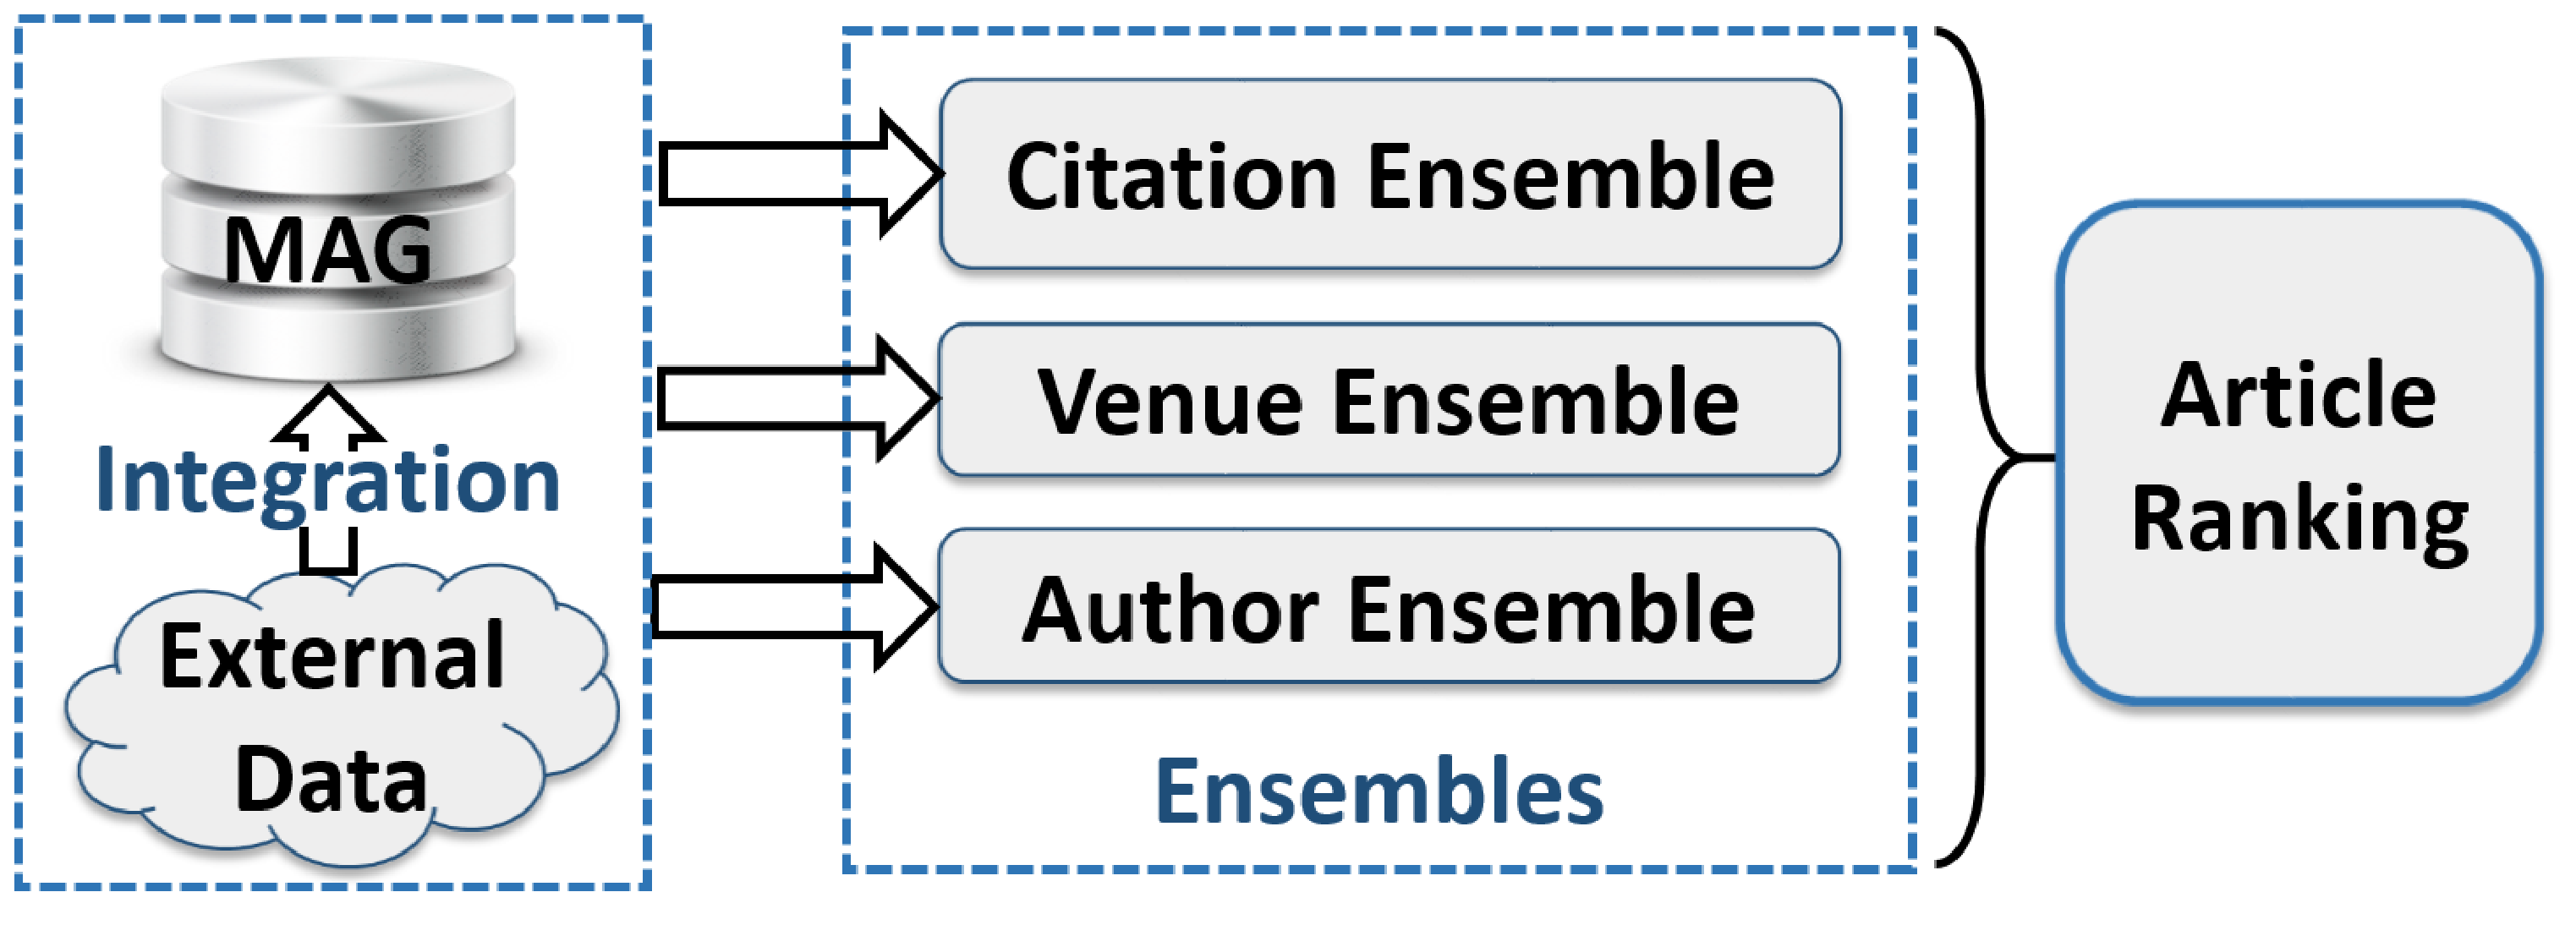
\includegraphics[scale=0.15]{fig/framework.eps}
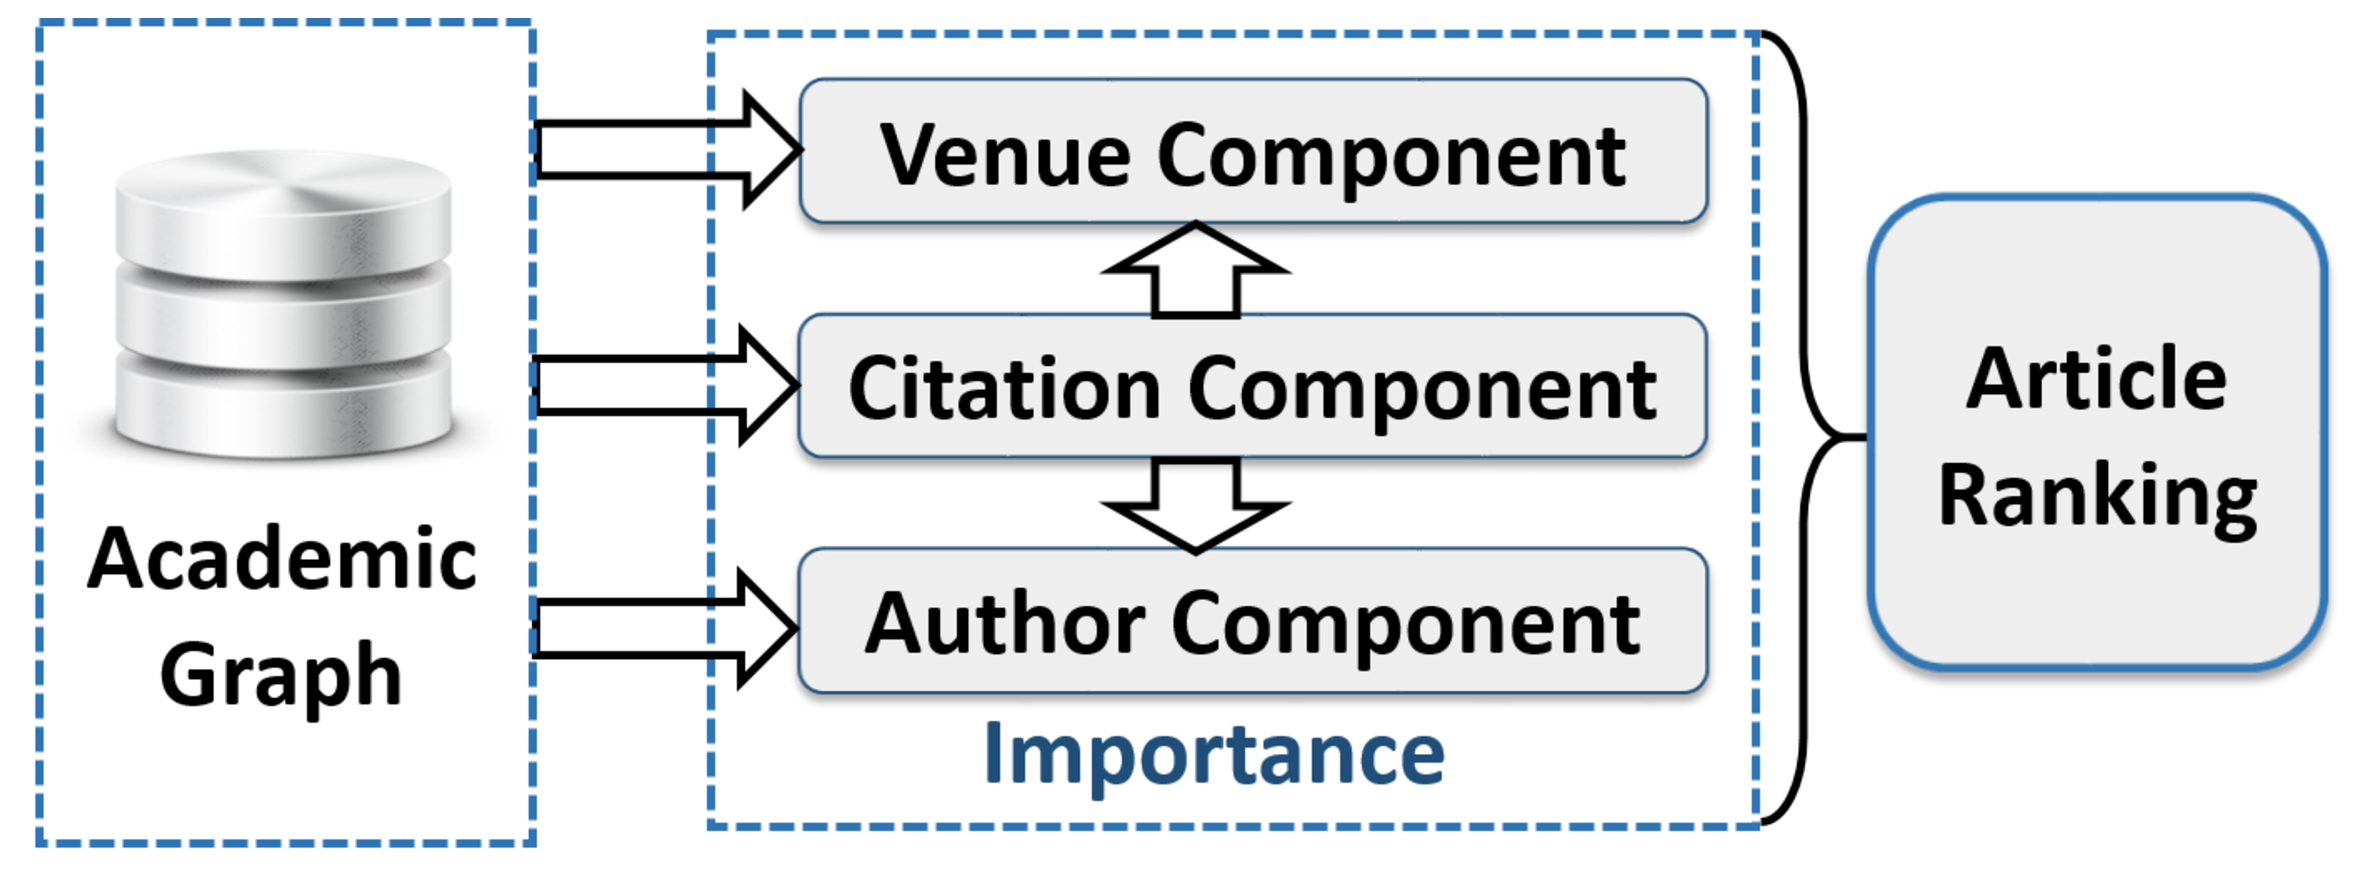
\includegraphics[scale=0.15]{fig/framework-lite-2.eps}
\vspace{-1ex}
\caption{\small Ranking model \ensemblerank} \label{fig-rankmodel}
\vspace{-3ex}
\end{figure}

\stitle{Venue component}.
The second component computes the importance of venues with their associated articles. As the importance of a venue  evolves with time, we treat the venue in each year individually, and its importance is the sum of importance in all individual years.


A {\em venue graph} $G^v(V^v, E^v)$ is firstly constructed using the citation information among venues such that (a) a node in $V^v$ represents a venue in a specific year, (b) a direct edge $(s,t)$ in $E^v$ denotes that there exist articles published in venue (in a specific year) $s$ citing articles published in venue (in a specific year) $t$, and (c) we use the {\em impact weight} $w_v(s,t)$ to denote the weight  from venues $s$ to $t$, which is the sum of the impact weights from articles published in $s$ to $t$, \ie

\vspace{-1ex}
\begin{small}
\begin{equation} \label{eq-infl-weights-v}
w_v(s,t)  = \sum_{u\in C(s), v\in C(t)} w(u,v).
\end{equation}
\end{small}
\noindent
Here, $C(s)$ and $C(t)$ are the sets of articles published in $s$ and $t$, respectively, and $w(u,v)$ is the impact weight of edge $(u, v)$ produced in the citation component.

The prestige of a venue in a specific year is computed using the impact weights and the update rule in Eq.~(\ref{eq-twpr}), and the popularity of a venue in a specific year is defined as the average popularity of its articles. The prestige and popularity are combined to derive the importance of a venue in a specific year in the same way as the citation component. Finally, the importance of a venue is treated as the {\em venue importance score} for all articles published in this venue.






\stitle{Author component}.
The author component computes the importance of authors with their published articles.
%
Similar to the venue component, we evaluate the importance of each author, and compute the average importance of the authors of an article as its {\em author importance score}.

%However, the resulting author citation graph to compute the prestige is typically too large to handle.
One way to do this is to construct an author citation graph  such that (a) a node represents an author, and (b) a direct edge $(s,t)$ denotes that there exist articles of author $s$ citing articles of author $t$. However, it is easy to see that for each citation, the corresponding two sets of authors are fully connected, which makes it computationally expensive to compute the prestige of authors on such an author citation graph with TWPageRank.

Hence, we choose to evaluate the prestige of an author with the average prestige of all articles published by the author. Similar to the venue component, the popularity of an author is  defined as the average popularity of her/his published articles. Finally, the prestige and popularity are combined to derive the importance along the same way as the citation component.

%, which can be directly obtained from the citation component,
%to evaluate the authority of that author.

\eat{
\stitle{Affiliation ensemble}.
Recall that articles in our data are also associated with affiliation information. Following the way of the venue or author ensemble, we can derive another ensemble, \ie affiliation ensemble. However, we argue that the use of affiliation ensemble may have negative effects since the correlation between the importance of an article and the average authority of its affiliation(s) is not as strong as others such like authors and venues. As shown by the experimental study in Section~\ref{sec-exp},  the incorporation of the affiliation ensemble impairs the ranking accuracy. Hence, we choose not to use the affiliation ensemble in our model.
}



%\subsection{Ranking with Importance}
%{\label{subsec-eerank}}


\stitle{Ranking with importance assembling}. The aforementioned importance is finally assembled to produce the final ranking, as illustrated in Fig.~\ref{fig-rankmodel}. Before assembling, each component is properly scaled such that the average importance scores of citations, venues and authors are the same.  Let the scaled importance scores of article $v$ be $R_c(v)$, $R_v(v)$, and $R_a(v)$ from the citation, venue and author components, respectively.
%
The final ranking score $R(v)$ is aggregated as follows:

\vspace{-1ex}
\begin{small}
\begin{equation} \label{eq-ensemble}
R(v) =  \alpha R_c(v) + \beta R_v(v) + (1 - \alpha - \beta) R_a(v).
\end{equation}
\end{small}
\noindent Here aggregating parameters $\alpha$ and $\beta$ and value $(1 - \alpha - \beta)$ regularize the contributions of the citation, venue and author information,
which make our model be able to fit to the various ranking scenarios. As will be seen in the experiments, our model performs well in two reasonable ranking scenarios by using quite different aggregating parameters, and, moreover, these parameters are indeed quite flexible to choose within a certain range.
Intuitively, these parameters indicate the intensity of the correlation between the importance of scholarly articles and the specific information.


\stitle{Remarks}. This work follows the graph-based formalization, and further develops efficient batch and incremental algorithms based on graphs for scholarly article ranking (Sections~\ref{sec-alg} \& \ref{sec-incAlg}). However, it is also possible to learn a discriminative model that directly optimizes certain loss functions for ranking, similar to \cite{Richardson06:BPR} for ranking Web pages.


%\subsection{Framework}
%\label{subsec-framework}

%Our ensemble enabled ranking model~\ensemblerank is illustrated in Fig.~\ref{fig-rankmodel}, which contains three distinct ensembles derived from academic graph data, \ie the citation ensemble, venue ensemble and author ensemble. The citation ensemble directly uses TWPageRank, while the other two are partially based on TWPageRank. Moreover, the citation ensemble also helps to derive the venue ensemble and author ensemble. These ensembles are further assembled to produce the final ranking.


%As illustrated in Fig.~\ref{fig-rankmodel}, external data is also exploited in \ewpr. How to collect and use external data will be introduced in the coming section.


\eat{
\stitle{Remarks}.
Traditional PageRank equally distributes the prestige of nodes, and PageRank based models suffer from the problem that older articles are preferred since they have accumulated a large number of citations~\cite{Li08TSRanking}, and TWPageRank based models alleviate the problem to a certain degree by lowering the impact weights of articles when they are cited after their peak time, \ie $T_u\geq Peak_v$. We further propose the venue and author ensembles to improve the ranking accuracy.
}



%\stitle{Remarks}.
%Recall that articles in our data are also associated with affiliation information. Following the way of the venue or author ensemble, we can derive another ensemble, \ie affiliation ensemble. However, we argue that the use of affiliation ensemble may have negative effects since the correlation between the importance of an article and the average authority of its affiliation(s) is not as strong as others such like authors and venues. As shown by the experimental study in Section~\ref{sec-exp},  the incorporation of the affiliation ensemble impairs the ranking accuracy. Hence, we choose not to use the affiliation ensemble in our model.


%our method used for author ensemble is both lightweight and effective, as will be shown in the experimental study.

%Two methods are used to evaluate the authority of venues and authors, respectively. We point out that the ensembles are quite flexible to the selection of these methods, and others may also be incorporated in the ensembles if appropriate.

\eat{
\subsection{Dealing with Missing Data}
\label{subsec-impl}

Data quality is one of the most challenging issues in large scale data management, especially for data from open domains and multiple sources, \eg the Microsoft Academic Graph (MAG)~\cite{Sinha15:MAG}.
The early version of MAG has $120$ million scholarly articles, among which we find that there are about $73$ million articles without references and about $77$ million ones without venues. The ranks of those articles with missing information are underestimated by our model \ewpr, since ensembles assign the minimum scores to articles. As a result, data missing seriously impairs the ranking accuracy.

As for references and venues, the later are easier to obtain, and each filled venue can have a direct and substantial impact on the article ranking, \ie $R_v(u)$ of Eq.~(\ref{eq-ensemble}). In contrast, a filled reference only has an indirect and slight impact. Hence, we decide to use external data to fill in missing venues.


%\subsection{Data Collecting}
%\label{subsec-datacraw}
\stitle{Data collecting}.
The raw external data is collected from publicly available Digital Libraries, such as IEEE Xplore ({\footnotesize http://ieeexplo-re.ieee.org/gateway/}),  PubMed ({\footnotesize http://www.ncbi.nlm.nih.gov/pub-med/}) and DBLP ({\footnotesize http://dblp.uni-trier.de/db/}). In total, we collect $2.8$ million articles with venue information as our external data, in which there are $57,000$ different venues.



%\subsection{Data Preprocessing}
%\label{subsec-dataprep}
\stitle{Data preprocessing}.
The venues in MAG are well processed, and are replaced by their series names. For example, {\em ``9th International Conference on Web Search and Data Mining, 2016''} is replaced with {\em ``Web Search and Data Mining''}. This makes it hard to directly link with the collected raw venue names. Hence, we preprocess raw venue names for the simplification of subsequent venue linking.
%
We first remove stop words such as {``on''} and common words like {``Conference''}, as well as years and some special characters from collected raw venue names. Then the same venues are merged, and the number of different venue names is reduced to $42,000$.

%\subsection{Data Linking}
%\label{subsec-datamap}
\stitle{Data linking}.
The final and also the most important step of filling missing venue information is to link each collected venue name to an existing one in MAG. Intuitively, linking based on name similarity is the most effective way such that two venues are linked if their names bear high similarity. We exploit the Jaro metric to evaluate the name similarity, which is based on the number and order of the common characters between two strings, and obtains good results in tasks such as record linkage and name matching~\cite{Cohen03strcompa}. Formally, a collected venue name is linked to an existing one in MAG if their Jaro similarity exceeds a pre-define threshold.

However, such a threshold is nontrivial to determine in practice. A high threshold can guarantee the accuracy of linked pairs, while only a tiny proportion of collected venue names are linked. On the other hand, a low threshold increases the number of linked pairs, which, in the same time, also introduces many errors. In order to reach a good balance between the number of linked pairs and the accuracy, we propose to combine another constraint on topic similarity of venues for linking, and only weaker filter conditions need be used in both constraints.

In MAG, fields of study (FOS) represent research topics of articles, such as {\em Web pages}, and {\em language technology}. Hence, we use FOS to evaluate the topic similarity of two venues. There are about $54,000$ FOS in MAG and most articles are assigned with two or three FOS. Let the set of FOS of each venue be the union of the sets of FOS of articles published in that venue. And the topic similarity of two venues based on FOS is defined as:
\begin{small}
\begin{equation} \label{eq-fos}
TS(s,t)=({|F_s\bigcap F_t|})/{\sqrt{|F_s|\cdot|F_t|}},
\end{equation}
\end{small}
\noindent in which $s$ and $t$ are two venues, and $F_s$ and $F_t$ are the sets of FOS of $s$ and $t$, respectively.

When we link a collected venue name, it is directly linked to the most similar one in terms of name similarity, if their Jaro similarity exceeds a high threshold $\lambda$. Otherwise, we first use the topic similarity constraint to select several candidates in MAG, \ie venues whose topic similarities with the collected venue exceed a threshold $\theta$. Intuitively, these candidates are in the similar fields of the collected one. We then select the most similar candidate in terms of name similarity as its linked venue, if their Jaro similarity exceeds another threshold $\phi$. Hence, the collected venue is linked to the one to which it is similar in terms of both topics and names.

In our model \ewpr, threshold $\lambda$ is set to $0.95$, while thresholds $\theta$ and $\phi$ need not be very high, which are $0.5$ and $0.7$, respectively. Finally, $6,000$ among the $42,000$ collected venues are linked, resulting in $340,000$ (about $12\%$) articles with enriched venue information. Note that a majority of the collected venue names are not valid venues, such as booktitles and names of workshops, and cannot be linked to any one in MAG.
}


